% The first argument is the \documentclass, which tells latex which template
% we're using to build this document. It's usually safe to just use "article".
\documentclass{article}

% include some packages...
\usepackage{fullpage} % change settings for a smaller margin
\usepackage{graphicx} % gives access to the \includegraphics commands
\usepackage{amsfonts}
\usepackage{float}
\usepackage{enumitem}
\usepackage{caption}
\usepackage[export]{adjustbox}
\usepackage{bookmark}
\graphicspath{{./images/}}

% tell Latex to use no paragraph indentation, but leave some space between
% paragraphs
\setlength{\parindent}{0in}
\setlength{\parskip}{0.1in}

\newcommand{\tib}[1]{\textit{\textbf{#1}}}
\newcommand{\code}[1]{\texttt{#1}}

% these commands merely set the values for the title/date/author; they don't put
% them in the document... see \maketitle below
\title{CS Department Automated Information Timeline \\ Iteration 1 Submission}
\date{February 5, 2024}
\author{Matthew Hays, Pawan Bhandari, Sarah Faron, Tim Klimpel}

% all document content goes between \begin{document} and \end{document}
\begin{document}

% this command actually creates the title/date/author in the document
\maketitle
\newpage
\tableofcontents
\listoffigures
\newpage

\section{Vision Statement}

\section{Requirements}
\subsection{Functional Requirements}
\subsection{Non-Functional Requirements}

\section{Glossary}

\section{Domain Model}

\Section{Use Cases}
\subsection{Use Case Diagram}
\begin{figure}[H]
    \centering
    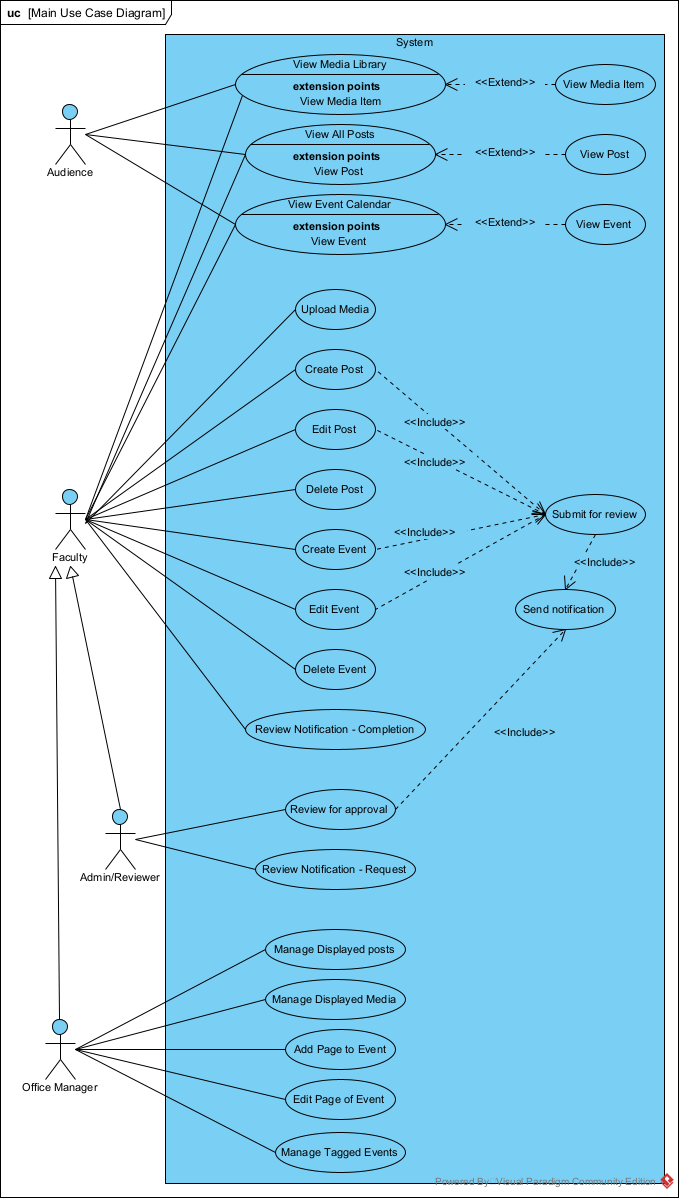
\includegraphics[width=0.8\textwidth]{images/UCD.png}
    \centering
    \caption{Use Case Diagram for CS Department Automated Information Timeline}
\end{figure}

\subsection{Use Cases}
There are a total of 16 use cases written at this stage in the project. Each team member was assigned 3 use cases to fully analyze. Each of these 12 use cases are written in fully-dressed form and accompanied by System Sequence Diagrams (SSDs) and Operations Contracts (OCs). The remaining 4 use cases are written in casual/brief form.

The assigned use cases are as follows:

\begin{center}
    \begin{tabular}{ | c | c | c | c | }
        \hline
        Bhandari & Faron & Hays & Klimpel \\
        \hline
        UC11 & UC05 & UC04 & UC15 \\
        \hline
        UC12 & UC06 & UC08 & UC16 \\
        \hline
        UC13 & UC07 & UC09 & UC01 \\
        \hline
    \end{tabular}
\end{center}

\subsubsection{UC01: View Media Library}
% \begin{figure}[H]
%     \centering
%     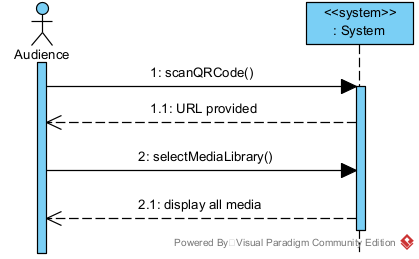
\includegraphics[width=0.8\textwidth]{images/SSD-UC01-ViewMediaLibrary.png}
%     \centering
%     \caption{System Sequence Diagram: View Media Library}
% \end{figure}
\subsubsection{UC02: View All Posts}
Brief.
\subsubsection{UC03: View Event Calendar}
Brief.
\subsubsection{UC04: Create Event}
% \begin{figure}[H]
%     \centering
%     \includegraphics[width=0.8\textwidth]{images/SSD-UC02-CreateEvent.png}
%     \centering
%     \caption{System Sequence Diagram: Create Event}
% \end{figure}
\subsubsection{UC05: Edit Event}
\begin{figure}[H]
    \centering
    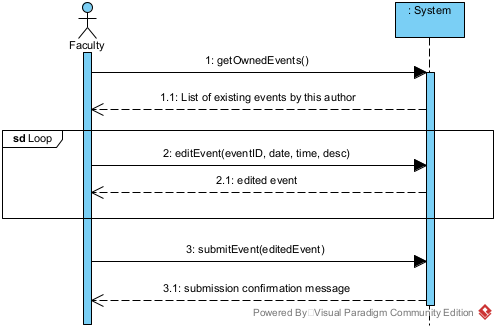
\includegraphics[width=0.8\textwidth]{images/SSD-UC05-EditEvent.png}
    \centering
    \caption{System Sequence Diagram: Edit Event}
\end{figure}
\subsubsection{UC06: Delete Event}
% \begin{figure}[H]
%     \centering
%     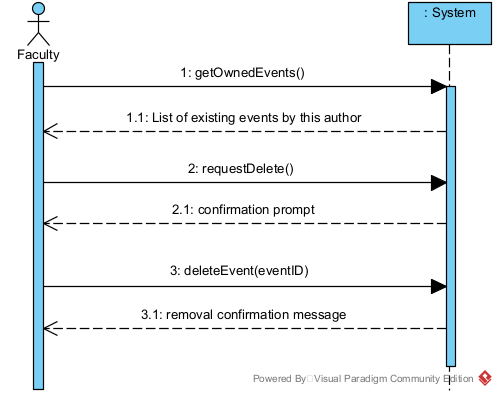
\includegraphics[width=0.8\textwidth]{images/SSD-UC06-DeleteEvent.png}
%     \centering
%     \caption{System Sequence Diagram: Delete Event}
% \end{figure}
\subsubsection{UC07: View Event}
% \begin{figure}[H]
%     \centering
%     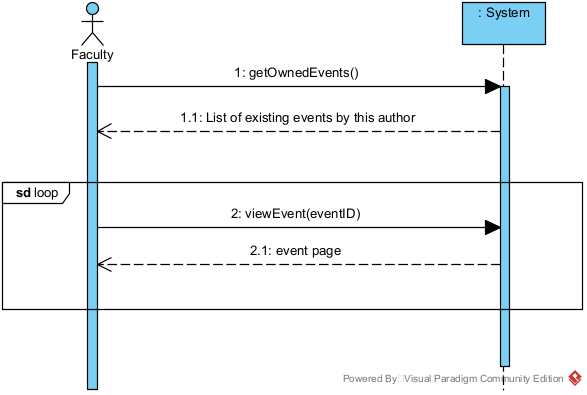
\includegraphics[width=0.8\textwidth]{images/SSD-UC07-ViewEvent.png}
%     \centering
%     \caption{System Sequence Diagram: View Event}
% \end{figure}
\subsubsection{UC08: Submit For Review}
\begin{figure}[H]
    \centering
    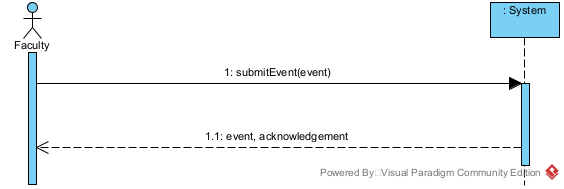
\includegraphics[width=0.8\textwidth]{images/SSD-UC08-SubmitForReview.png}
    \centering
    \caption{System Sequence Diagram: Submit For Review}
\end{figure}
\subsubsection{UC09: Review For Approval}
% \begin{figure}[H]
%     \centering
%     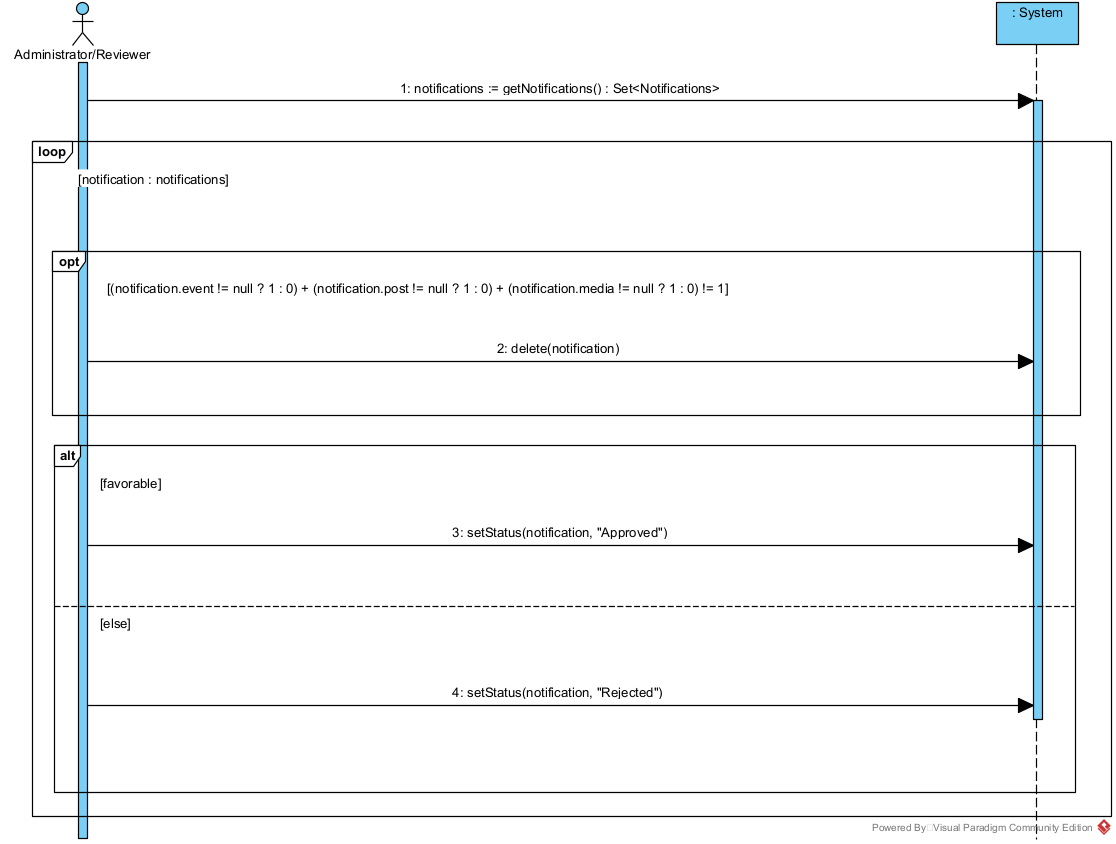
\includegraphics[width=0.8\textwidth]{images/SSD-UC09-ReviewForApproval.png}
%     \centering
%     \caption{System Sequence Diagram: Review For Approval}
% \end{figure}
\subsubsection{UC10: Create Post}
Brief.
\subsubsection{UC11: Edit Post}
\begin{figure}[H]
    \centering
    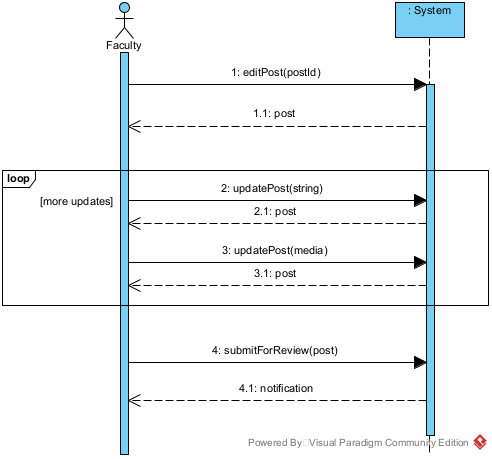
\includegraphics[width=0.8\textwidth]{images/SSD-UC11-EditPost.png}
    \centering
    \caption{System Sequence Diagram: Edit Post}
\end{figure}
\subsubsection{UC12: Delete Post}
% \begin{figure}[H]
%     \centering
%     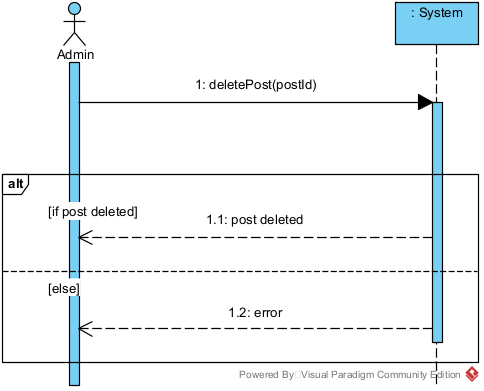
\includegraphics[width=0.8\textwidth]{images/SSD-UC12-DeletePost.png}
%     \centering
%     \caption{System Sequence Diagram: Delete Post}
% \end{figure}
\subsubsection{UC13: View Post}
% \begin{figure}[H]
%     \centering
%     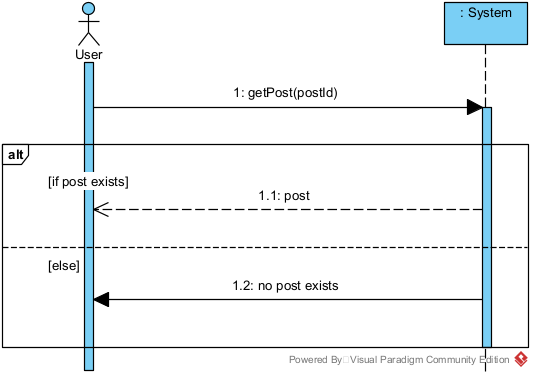
\includegraphics[width=0.8\textwidth]{images/SSD-UC13-ViewPost.png}
%     \centering
%     \caption{System Sequence Diagram: View Post}
% \end{figure}
\subsubsection{UC14: Update HTML on Page}
Brief.
\subsubsection{UC15: Manage Displayed Posts}
% \begin{figure}[H]
%     \centering
%     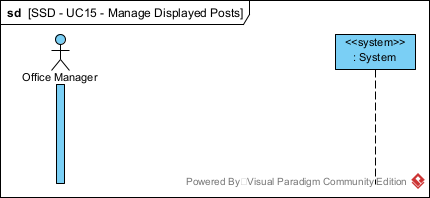
\includegraphics[width=0.8\textwidth]{images/SSD-UC15-ManageDisplayedPosts.png}
%     \centering
%     \caption{System Sequence Diagram: Manage Displayed Posts}
% \end{figure}
\subsubsection{UC16: Manage Displayed Media}
\begin{figure}[H]
    \centering
    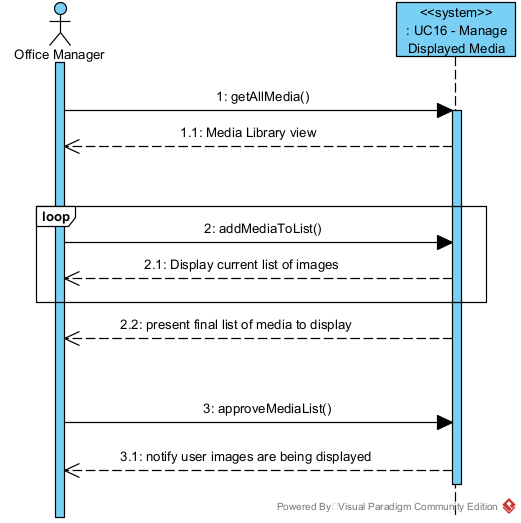
\includegraphics[width=0.8\textwidth]{images/SSD-UC16-ManageDisplayedMedia.png}
    \centering
    \caption{System Sequence Diagram: Manage Displayed Media}
\end{figure}

\section{Activity Diagram: Create Event}
\begin{figure}[H]
    \centering
    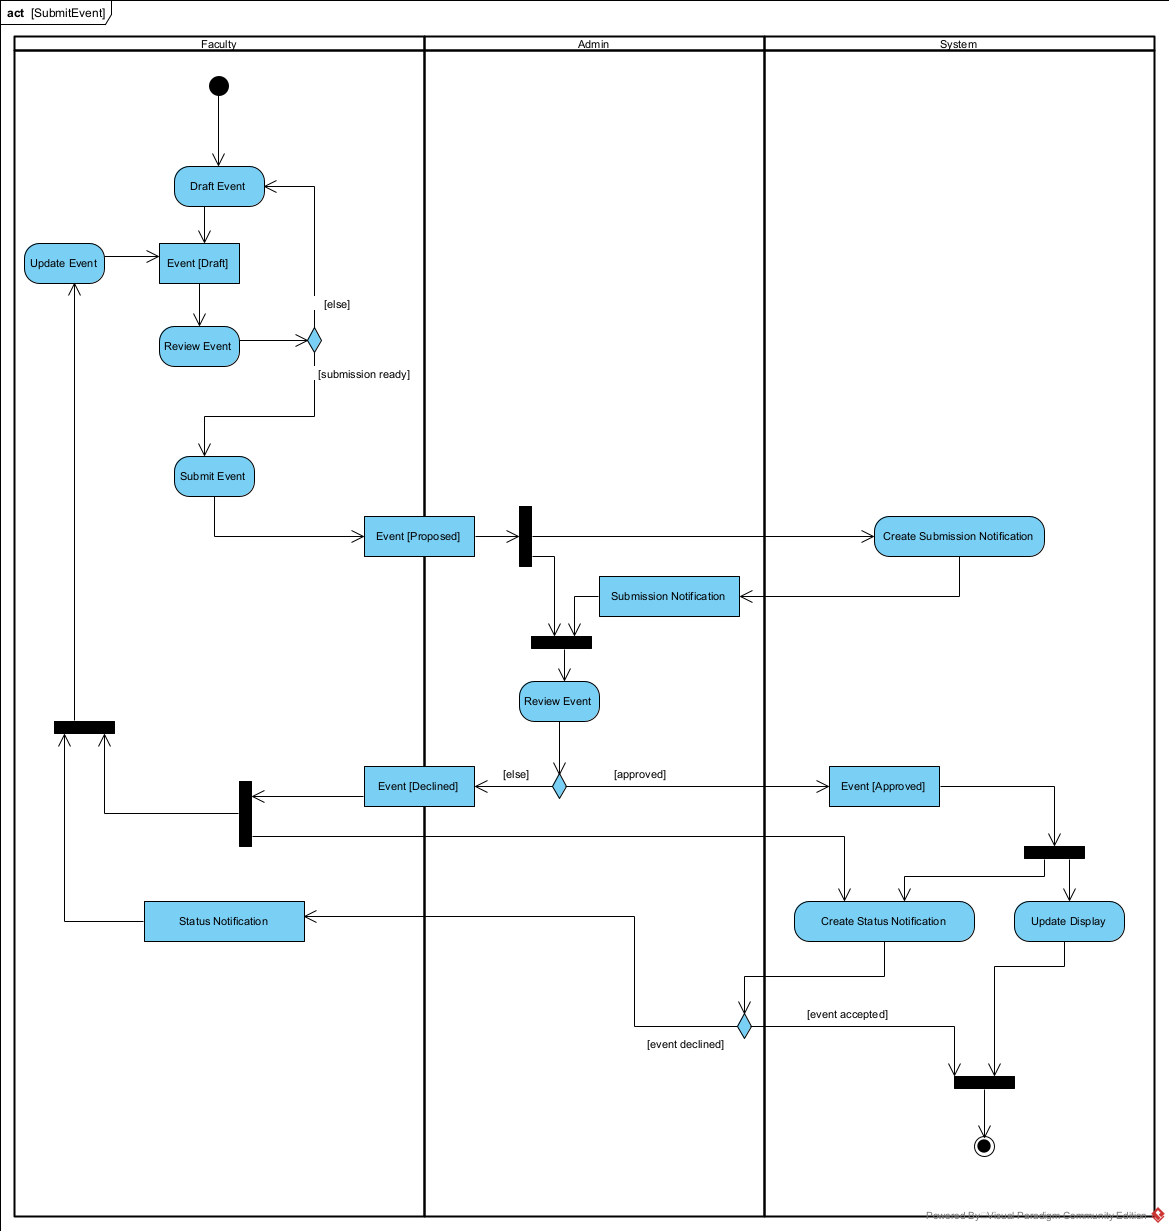
\includegraphics[width=.98\textwidth]{images/SubmitEvent.png}
    \centering
    \caption{Activity Diagram: Create Event}
    \label{fig:activityDiagram}
\end{figure}

\section{Wireframes}
\subsection{TV}
% \begin{figure}[H]
%     \centering
%     \includegraphics[width=0.8\textwidth]{images/wireframe-TV.png}
%     \centering
%     \caption{Wireframe: TV}
% \end{figure}

\subsection{Website}
% \begin{figure}[H]
%     \centering
%     \includegraphics[width=0.8\textwidth]{images/wireframe-website.png}
%     \centering
%     \caption{Wireframe: Website}
% \end{figure}

\end{document}
